\newpage 
\section{Industry Analysis}
\begin{wrapfigure}{r}{0.4\textwidth}
    \centering
    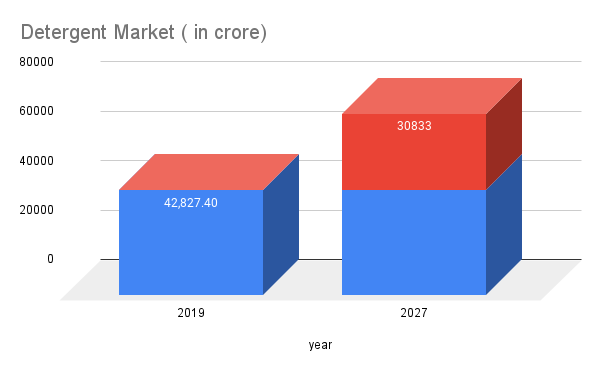
\includegraphics[width=0.9\linewidth]{images/Detergent Market.png}
    \caption{Detergent Market ( in crore)}
    \label{fig:hul_logo}
\end{wrapfigure}
The India detergents market was valued at INR 42,827.4 crore in 2019 and is projected to reach INR 73,660.4 crore by 2027; it is expected to grow at a CAGR of 7.0\% from 2020 to 2027. Increasing consumer awareness about enhancing health and quality of living; and rising disposable income and consumer expenditure on personal hygiene products, resulting into high consumption of products such as fabric softeners, hair and body care products, sanitizers, and disinfectants have been the factors driving the market growth in India.

\subsection{Relative Market Share}
\begin{figure}[h]
    \centering
    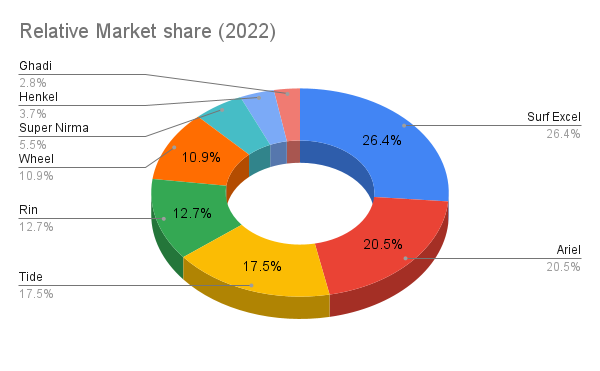
\includegraphics[width=0.9\textwidth]{images/Relative Market share (2022).png}
    \caption{Relative Market share (2022)}
    \label{fig:BCG Matrix}
  \end{figure}
In the laundry detergent market, Surf Excel leads with a substantial relative market share of 26.36\%, followed by Ariel at 20.45\% and Tide at 17.54\%. Rin and Wheel hold notable positions with 12.73\% and 10.91\%, respectively. Super Nirma, Henkel, and Ghadi have comparatively smaller shares at 5.45\%, 3.73\%, and 2.83\%, respectively. The data reflects Surf Excel's dominance in the segment, with other brands holding varying market positions. This distribution emphasizes the competitive landscape, illustrating the preferences of consumers in the laundry detergent market.

\subsection{Industry Analysis using Porter's Five Forces Model}
\begin{figure}[H]
    \centering
    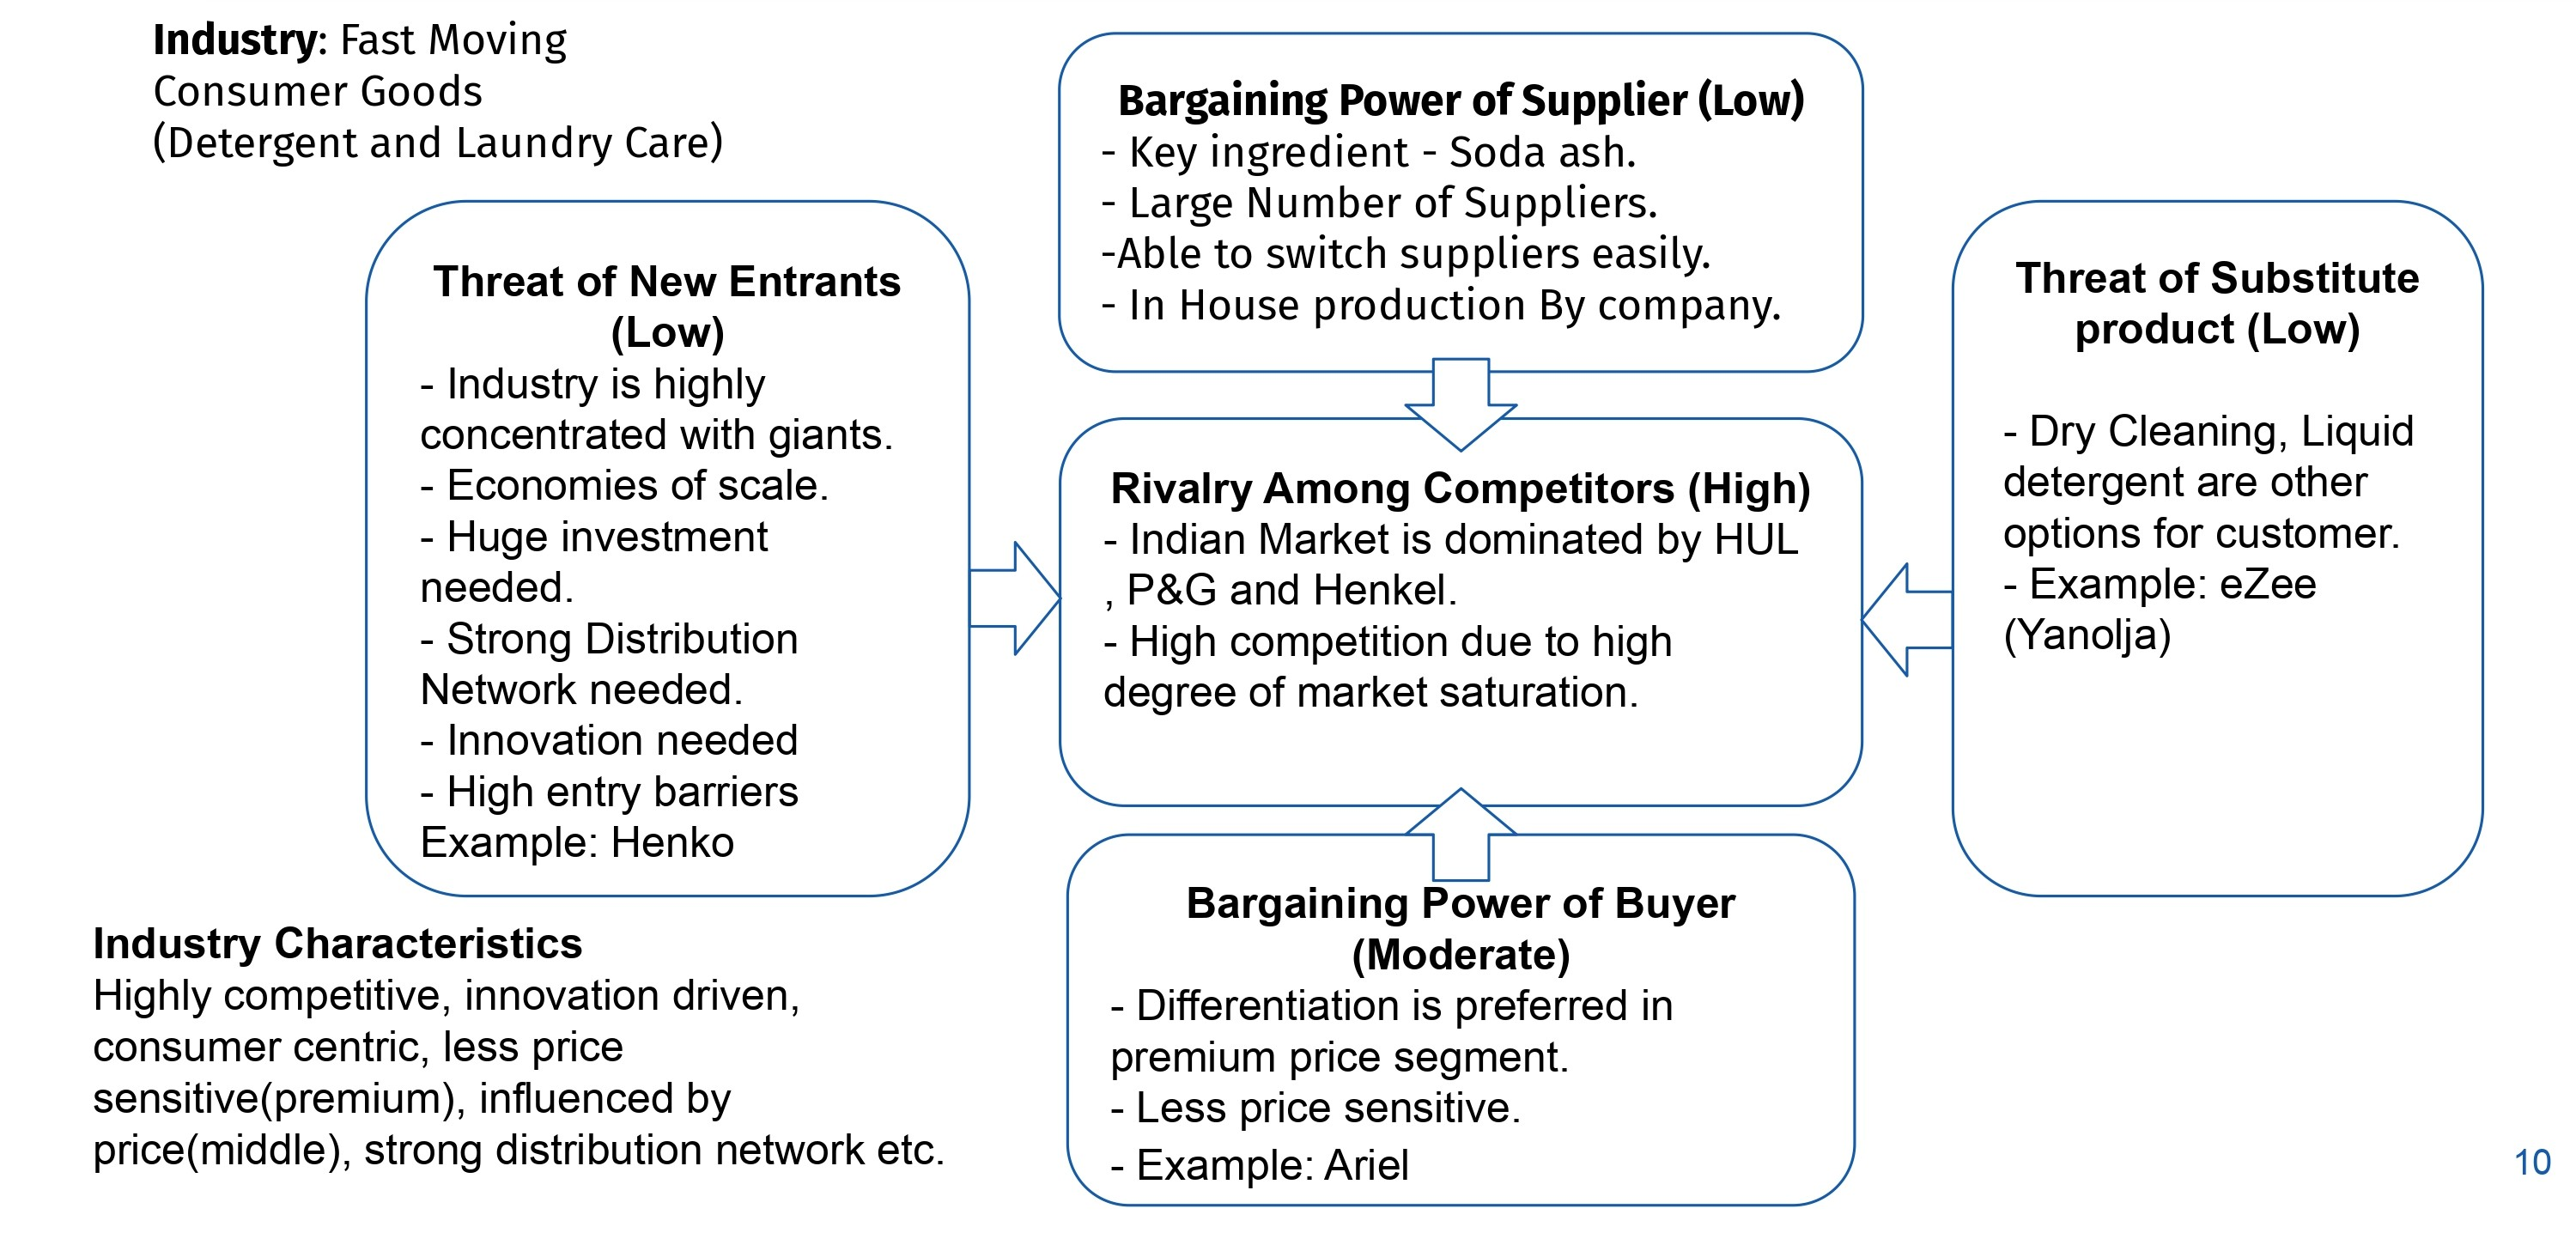
\includegraphics[width=0.9\textwidth]{images/Porters Model.jpg}
    \caption{Industry Analysis (Porter’s Model)}
    \label{fig:BCG Matrix}
  \end{figure}
\subsubsection{Industry Characteristics}
The fast-moving consumer goods (FMCG) industry, particularly in the detergent and laundry care segment, exhibits distinctive features. It is characterized by high competitiveness, driven by constant innovation and a consumer-centric approach. The industry shows a spectrum of consumer sensitivity, with a significant premium sector indicating a lesser degree of price sensitivity. A robust distribution network plays a crucial role in reaching consumers efficiently.

\subsubsection{Threat of New Entrants (Low)}
\begin{itemize}
  \item The threat of new entrants into the detergent and laundry care industry is low, primarily due to several barriers.
  \item The industry is highly concentrated, dominated by major players like HUL, P\&G, and Henkel.
  \item Giants benefit from economies of scale, making it challenging for new entrants to achieve cost efficiencies.
  \item Substantial investments are required for manufacturing facilities, marketing, and research and development.
  \item A strong distribution network is essential for success, creating high entry barriers.
  \item Innovation is a key competitive factor, requiring significant resources for new entrants.
  \item Example: High entry barriers seen in the case of Henko.
\end{itemize}

\subsubsection{Bargaining Power of Suppliers (Low)}
\begin{itemize}
  \item Suppliers in the detergent and laundry care industry, particularly providing key ingredients like soda ash, have relatively low bargaining power.
  \item The industry has a large number of suppliers, providing companies with flexibility to switch suppliers easily.
  \item Some companies opt for in-house production, reducing dependency on external suppliers.
  \item Suppliers lack significant leverage over manufacturers, allowing companies to negotiate favorable terms and maintain control over the supply chain.
\end{itemize}

\subsubsection{Rivalry Among Competitors (High)}
\begin{itemize}
  \item Rivalry among competitors in the detergent and laundry care industry is intense due to the dominance of major players like HUL, P\&G, and Henkel.
  \item The market is saturated, and key players continually strive for innovation to gain a competitive edge.
  \item Price wars and marketing strategies are common as companies vie for market share.
  \item The strong brand presence and consumer loyalty enjoyed by established companies make it challenging for new entrants to disrupt the market.
\end{itemize}

\subsubsection{Bargaining Power of Buyers (Moderate)}
\begin{itemize}
  \item Buyers in the detergent and laundry care industry exhibit moderate bargaining power.
  \item Differentiation is preferred in the premium price segment, with consumers generally less price-sensitive.
  \item Established brands like Ariel can command premium prices based on perceived quality and features.
  \item Buyers have the flexibility to switch between brands, especially in the middle price range, contributing to a moderate level of bargaining power.
\end{itemize}

\subsubsection{Threat of Substitute Products (Low)}
\begin{itemize}
  \item The threat of substitute products in the detergent and laundry care industry is relatively low.
  \item Alternatives like dry cleaning and liquid detergents exist, but the core demand for traditional detergent products remains robust.
  \item Substitutes might cater to specific niche preferences, but the widespread use of conventional detergents limits the impact of substitute products.
  \item Example: eZee by Yanolja faces a low threat despite being an alternative due to the entrenched use of traditional detergents.
\end{itemize}

In conclusion, Porter's Five Forces analysis reveals that the detergent and laundry care industry is characterized by high barriers to entry, intense competition among established players, and moderate bargaining power of buyers. The low threat of substitutes and the low bargaining power of suppliers contribute to the overall stability of the industry. This analysis aids in understanding the competitive dynamics and strategic considerations within the FMCG sector, guiding companies in making informed decisions for sustained success.
\section{SWOT Analysis}

\subsection{Strengths}

Surf Excel's market leadership in the premium segment is a significant strength, indicating its strong brand recognition and consumer trust. The heavy investment in Research and Development (R\&D), backed by a team of 700+ scientists and a global patent portfolio of 20,000, reflects a commitment to innovation and product quality. The robust distribution network facilitated by Hindustan Unilever Limited (HUL) provides a competitive advantage, ensuring widespread availability. An aggressive marketing strategy and a focus on premiumization further strengthen Surf Excel's position in the market.

\subsection{Weaknesses}

The slightly higher price of Surf Excel may limit its reach to the mass market, potentially affecting market share. Limited product awareness in rural markets poses a challenge, requiring targeted marketing efforts. Environmental concerns, likely related to the use of chemicals and energy-intensive manufacturing, present a vulnerability that aligns with evolving consumer preferences for sustainable products.

\subsection{Internal Logic}

Surf Excel's dominant market share of 26.4\% in the detergent segment (S1) signifies its stronghold and popularity. The substantial investment in R\&D (S2) positions the brand at the forefront of innovation. The marketing strategy (S4) aligns with the brand's ethos of embracing childhood experiences.

To address weaknesses, implementing lean manufacturing practices (W1) can optimize production processes, potentially reducing costs and addressing affordability concerns. Enhancing environmental sustainability measures (W3) is crucial for mitigating negative impacts, aligning with growing consumer preferences for eco-friendly products.

In conclusion, Surf Excel's strengths lie in its market leadership, R\&D investment, distribution network, and marketing strategy. Addressing weaknesses through cost optimization and sustainable practices will be vital for long-term competitiveness in the dynamic detergent market.


\subsection{Threats:}

The detergent sector poses challenges with low-profit margins (T1), impacting Hindustan Unilever Limited's (HUL) capacity for significant returns on investments. This limitation could hinder innovation, marketing endeavors, and overall expansion efforts. Intense competition from existing and new players (T2) heightens the risk of price wars, aggressive marketing, and product proliferation, challenging HUL's dominance. Regulatory compliances, especially from the Central Drugs Standard Control Organization (CDSCO) (T3), introduce the risk of negative publicity and potential legal actions, particularly concerning environmental and health concerns. Rising raw material and transportation costs (T4) add economic pressure, impacting the cost-effectiveness of production and distribution.

\subsection{Opportunities:}

The detergent sector presents opportunities for growth, driven by rapid market expansion into rural areas (O1). The increasing accessibility of consumer goods in rural India benefits HUL's distribution network. Adapting to changing customer needs and lifestyles (O2) aligns with the growing demand for eco-friendly and sustainable household products. The anticipated 7\% growth in the Indian detergent market (O3) provides HUL with the chance to capitalize on a dynamically expanding market. The emergence of new online shopping platforms and digital marketplaces (O4) offers additional sales channels for Surf Excel, tapping into the evolving landscape of consumer behavior.

\subsection{External Logic:}

The rapid expansion of rural retail, including kirana stores and small supermarkets (O1), enhances the accessibility of consumer goods in rural India, aligning with HUL's market distribution. The growing demand for eco-friendly products (O2) and increased awareness among consumers favor Surf Excel's commitment to sustainability. The emergence of online shopping platforms (O3) provides new avenues for sales, adapting to changing consumer preferences.

In summary, while threats such as low-profit margins, intense competition, and regulatory compliances exist, opportunities in market growth, adapting to consumer needs, and the emergence of new marketplaces offer avenues for Hindustan Unilever Limited to navigate challenges and sustain its competitive edge in the dynamic detergent sector.

\section{Marketing Campaign}

\subsection{Positioning - Superiority via Value Perception and Emotional Engagement
}
In the face of a price-led threat from Nirma, Surf Excel devised a brilliant marketing strategy that not only countered the competition but also elevated its brand positioning. Instead of engaging in a self-destructive price war, Surf Excel focused on emphasizing its superior value proposition, appealing to the discerning Indian homemaker.

The iconic "Lalitaji" campaign epitomized this approach. Lalitaji, the quintessential value-conscious yet savvy homemaker, represented the target audience who sought products that offered the best value for their money, not necessarily the lowest price. The campaign resonated with Indian consumers, establishing Surf Excel as a brand that understood their needs and aspirations.

\subsection{"Daag Acche Hain" - A Purposeful Brand Shift}
Building upon its success, Surf Excel embarked on a transformative journey with its "Daag Acche Hain" campaign. This groundbreaking campaign marked a paradigm shift in the detergent industry, moving away from the traditional focus on stain removal and towards a more purposeful brand message.

The campaign celebrated the inherent value of childhood experiences, highlighting the importance of allowing children to explore and learn, even if it means getting their clothes dirty. This message resonated deeply with Indian parents, who often struggle to balance the desire to protect their children with the need to let them grow and learn through their own experiences.

Surf Excel's willingness to address a broader societal issue, rather than just focusing on product features, solidified its position as a brand that understood and cared about its consumers' lives. The campaign's success demonstrated the power of purpose-driven marketing and its ability to connect with consumers on an emotional level.

\subsection{Product Innovation - Delivering Value through Continuous Innovation
}
Surf Excel has consistently supported its brand positioning with a commitment to continuous product innovation. The brand was the first to introduce liquid laundry detergent in India, demonstrating its ability to anticipate and adapt to changing consumer needs.

Surf Excel's approach to innovation has always been focused on adding value for consumers, rather than simply cutting prices. The brand's innovative products have consistently delivered superior performance, convenience, and value, further strengthening its position as a premium detergent brand.

Surf Excel's marketing campaigns and product innovation strategies have played a pivotal role in its success. By consistently delivering value through its products and campaigns, Surf Excel has established itself as a trusted and beloved brand in Indian households.

\section{Conclusion}


In conclusion, Surf Excel's enduring success in the detergent market is intricately linked to its premiumization strategy, a path it has navigated through market fluctuations. While this approach has proven effective, occasionally sparking controversy, such as the backlash to its 2019 Holi ad, it underscores the brand's bold positioning and willingness to push boundaries. The inadvertent call for boycotting Microsoft Excel instead of Surf Excel, albeit humorous, highlights the brand's impact on popular culture.

Nevertheless, Surf Excel's deliberate premiumization, coupled with strategic marketing and continuous product innovation, has yielded remarkable results. Achieving billion-dollar status and securing undisputed market leadership in its segment showcase the dividends of this approach. The brand's growth is a testament to the potency of patient brand-building, emphasizing the importance of foundational elements and a commitment to constant evolution. Surf Excel's journey serves as a case study in effective marketing strategies, demonstrating how a well-executed premiumization strategy, grounded in innovation and consistent evolution, can propel a brand to sustained success.